% !TeX root = ../../../01_git-vorgehensmodelle.tex

\subsection{Branching-Strategien}
\label{sec:workflows:branching}

In größeren Projekten können sich Änderungen an einem Feature schnell auf andere Bereiche der Software auswirken. Zudem können Features, die sich in der Entwicklung befinden, instabilen Code erzeugen~\cite{sorin_dumitrescu_what_2021}. Vor allem wenn viele Entwickler:innen zur gleichen Zeit an unterschiedlichen Stellen der Software Änderungen vornehmen, stellt dies eine Herausforderung dar.

Um eine stabile Codebasis zu erhalten und zu verhindern, dass sich die Entwickler:innen gegenseitig behindern, arbeiten die meisten Entwicklungsteams mit unterschiedlichen Branching\hyp Strategien. Durch einen Branch wird innerhalb des Repositories eine Kopie der Codebasis zu diesem Zeitpunkt erstellt. Auf dem Branch können anschließend Features entwickelt oder andere Änderungen eingepflegt werden~\cite{atlassian_hintergrundwissen_2023}. Änderungen in einem Branch haben keine Auswirkungen auf andere Branches. Somit können sich die Entwickler:innen nicht gegenseitig stören~\cite{atlassian_hintergrundwissen_2023}. Branches können nach Abschluss mit einem Merge wieder zusammengeführt werden.

In den folgenden Abschnitten werden drei häufig verwendete Branching\hyp Strategien vorgestellt. Diese können optional parallel verwendet werden und unterscheiden sich hauptsächlich darin, wie und wofür Branches erstellt und wieder zusammengeführt werden.


\subsubsection{Feature\hyp Branching\hyp Strategie}

Bei der Verwendung der \emph{Feature\hyp Branching}\hyp Strategie, werden neue Features nicht mehr auf dem Haupt\hyp Branch entwickelt. Stattdessen wird für jedes neue Feature ein dedizierter Branch erstellt~\cite{atlassian_feature_2023}. Ein Beispiel für diese Vorgehensweise ist in \autoref{fig:task_branch:feature} dargestellt.

\begin{figure}
    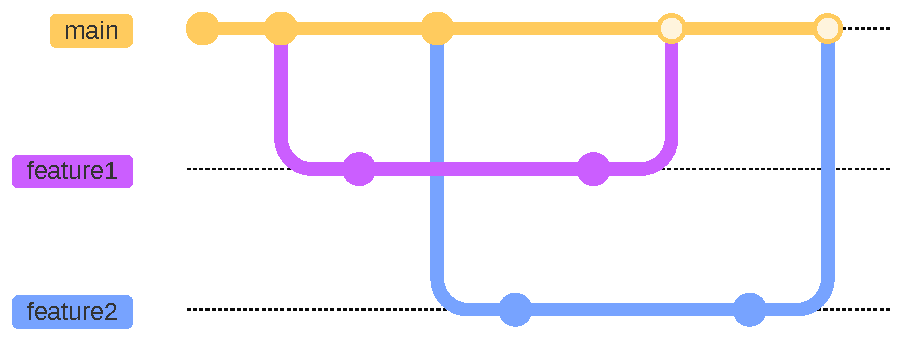
\includegraphics[width=0.45\textwidth]{assets/diagrams/task_branch/feature-branch.pdf}
    \caption{Zwei Feature\hyp Branches}
    \label{fig:task_branch:feature}
    \Description{In der Abbildung ist ein Git\hyp Graph dargestellt, welcher die Branches main, feature1 und feature2 beinhaltet. Letztere werden jeweils von main abgezweigt und schließlich dorthin zurück integriert.}
\end{figure}

Dabei ist zu erkennen, wie zwei Feature\hyp Branches -- \texttt{feature1} und \texttt{feature2} -- vom Haupt\hyp Branch \texttt{main} erstellt werden. Auf beiden Branches wird anschließend parallel das jeweilige Feature entwickelt und nach Abschluss per Merge in \texttt{main} übertragen. Dadurch wird der zuvor erwähnte instabile Code, der bei der Entwicklung neuer Features entstehen kann, vom Haupt\hyp Branch isoliert. Dieser behält somit eine stabile Codebasis~\cite{sorin_dumitrescu_what_2021}.

Ein weiterer Vorteil der Feature\hyp Branching\hyp Strategie ist, dass bevor ein Merge durchgeführt wird, eine Pull Request erstellt werden kann. Eine Pull Request (häufig auch als \emph{Merge Request} bezeichnet) ist keine Funktion von Git selbst, wird jedoch von bekannten Git\hyp Hosting\hyp Services wie GitHub, GitLab oder Bitbucket bereitgestellt~\cite{heddings_what_2021}.

Bei einer \emph{Pull Request} wird eine Anfrage für den Merge eines Branches in einen anderen gestellt. Andere Entwickler:innen können anschließend an dieser Stelle vorab den Code überprüfen, Feedback geben und den Merge genehmigen~\cite{atlassian_feature_2023}. Diese gegenseitige Kontrolle führt zu einer höheren Codequalität, da Bugs und andere Fehler früher entdeckt werden können~\cite{pullrequest_why_2023}. Zahlreiche Git\hyp Hosting\hyp Services ermöglichen daher das Erstellen von Branch\hyp Schutzregeln. Diese Regeln können bspw. erzwingen, dass Änderungen auf bestimmten Branches ausschließlich über Pull Requests möglich sind~\cite{benvegnu_best_2020}.

Ein großer Nachteil der Feature\hyp Branching\hyp Strategie sind leicht auftretende Merge\hyp Konflikte~\cite{sorin_dumitrescu_what_2021}. Diese treten auf, wenn bei der Entwicklung unterschiedlicher Features Änderungen an denselben Stellen im Code vorgenommen wurden. Vor einem Merge müssen die Konflikte aufgelöst werden.

Da die Unterschiede zwischen Feature\hyp Branches und dem Haupt\hyp Branch immer größer werden, je länger diese existieren, steigt mit der Zeit auch die Wahrscheinlichkeit dafür, dass große und komplexe Merge\hyp Konflikte entstehen. Um dies zu vermeiden, sollten Feature\hyp Branches so früh wie möglich durch einen Merge in den Haupt\hyp Branch übernommen werden~\cite{sorin_dumitrescu_what_2021}.


\subsubsection{Release\hyp Branching Strategie}

Bei der \emph{Release\hyp Branching}\hyp Strategie wird vor jedem Release ein neuer Branch aus dem Haupt\hyp Branch erstellt. Auf diesem Branch können letzte Bugs behoben und Anpassungen vorgenommen werden ohne damit die Entwicklung der anderen Features zu stören ~\cite{tucker_basics_2023}. Der Release\hyp Branch bleibt dabei als langlebiger Branch dauerhaft erhalten. Dadurch können parallel laufende Versionen unterstützt werden~\cite{hart_besten_2020}. Ein Beispiel für diese Vorgehensweise ist in \autoref{fig:task_branch:release} dargestellt.

\begin{figure}
    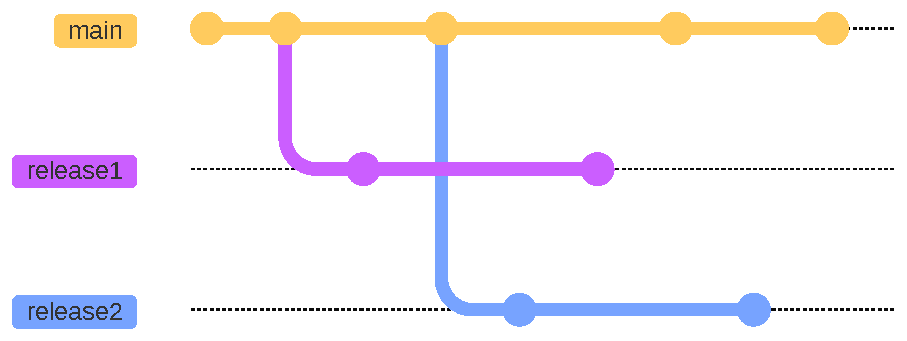
\includegraphics[width=0.45\textwidth]{assets/diagrams/task_branch/release-branch.pdf}
    \caption{Zwei Release\hyp Branches}
    \label{fig:task_branch:release}
    \Description{In der Abbildung ist ein Git\hyp Graph dargestellt, welcher die Branches main, release1 und release2 beinhaltet. Letztere werden jeweils von main abgezweigt und bleiben für den Rest der Entwicklung erhalten.}
\end{figure}

Dabei ist zu erkennen, dass der Branch \texttt{release1} für den ersten Release erstellt wird. Danach wird auf dem \texttt{main}\hyp Branch weiterentwickelt, ohne dass der \texttt{release1}-Branch gelöscht wird. Anschließend kommt es zu einem zweiten Release, wobei jeder Release einen zugehörigen Branch behält. Zudem ist zu erkennen, dass auf beiden Release\hyp Branches weitere Änderungen hinzugefügt werden, die für den Release notwendig sind.
Für Projekte, in denen mehrere Versionen parallel unterstützt werden sollen, ist dieses Vorgehen notwendig, da durch eigene Release\hyp Branches spezifische Probleme der jeweilige Version später leicht behoben werden können~\cite{hart_besten_2020}.

Falls gewünscht, können die Änderungen auf dem Release\hyp Branch in den Haupt\hyp Branch übernommen werden. Dazu existieren unterschiedliche Vorgehensweisen. Zum einen können die Änderungen durch eine Pull\hyp Request bzw. Merge in den Haupt\hyp Branch übernommen werden. Der Release\hyp Branch muss dabei jedoch auch nach dem Merge erhalten bleiben~\cite{tucker_basics_2023}. Alternativ können jedoch auch nur die gewünschten Änderungen per Cherry\hyp Pick in den Haupt\hyp Branch übernommen werden~\cite{vijayma_git_2022}.

Ein Nachteil der Release\hyp Branching\hyp Strategie besteht darin, dass die Arbeit mit vielen parallelen Branches die Pflege des Repositories erschwert. So müssen Hotfixes häufig per Merge oder Cherry\hyp Pick in mehrere Release\hyp Branches übernommen oder sogar für unterschiedliche Releases gesondert entwickelt werden~\cite{hart_besten_2020}.


\subsubsection{Task\hyp Branching\hyp Strategie}

Da die Koordinierung vieler Aufgaben in großen Projekten schnell unübersichtlich werden kann, wird häufig Tracking\hyp Software für Vorgänge verwendet. Dabei wird für jedem Vorgang ein Ticket (bspw. in Jira) oder ein Issue (bspw. in GitLab oder GitHub) erstellt. Bei der Verwendung der Task\hyp Branching\hyp Strategie wird für jeden dieser Vorgänge ein eigener Branch erstellt~\cite{atlassian_hintergrundwissen_2023}. Der Vorgangsschlüssel aus der Vorgangs\hyp Tracking\hyp Software muss dabei in den Branch\hyp Namen integriert werden. Dadurch kann jeder Branch schnell einem Ticktet zugeordnet werden~\cite{atlassian_hintergrundwissen_2023}. Ein Beispiel für diese Vorgehensweise ist in \autoref{fig:task_branch:task} dargestellt. 

\begin{figure}
    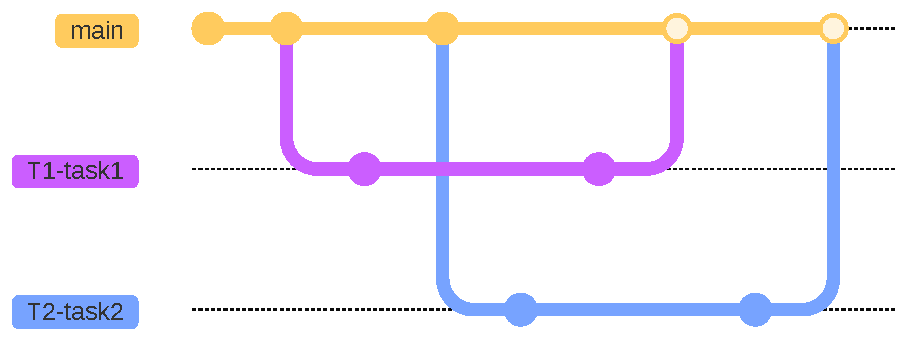
\includegraphics[width=0.45\textwidth]{assets/diagrams/task_branch/task-branch.pdf}
    \caption{Zwei Task\hyp Branches}
    \label{fig:task_branch:task}
    \Description{In der Abbildung ist ein Git\hyp Graph dargestellt, welcher die Branches main, task1 und task2 beinhaltet. Letztere werden jeweils von main abgezweigt und schließlich dorthin zurück integriert. T1 und T2 stehen dabei für den Schlüssel der zugehörigen Vorgänge}
\end{figure}

Hierbei ist zu erkennen, dass nacheinander die beiden Task\hyp Branches \texttt{T1-task1} und \texttt{T2-task2} erstellt werden. Der Präfix \texttt{T1} und \texttt{T2} im Namen beider Branches steht für den Schlüssel der zugehörigen Vorgänge.
Durch den Vorgangsschlüssel im Namen des Branches ist schnell ersichtlich, für welche Vorgänge schon ein Branch erstellt wurde und welcher Vorgang zu einem Branch gehört. Git\hyp Hosting\hyp Services wie GitHub erstellen zudem eine automatische Verlinkung sobald der Vorgangsschlüssel im Namen des Branches verwendet wird~\cite{github_inc_autolinked_2023}.


\subsubsection{Fazit}

Besonders in großen Projekten, in denen viele Entwickler:innen parallel an unterschiedlichen Features arbeiten, können Branching\hyp Strategien dabei helfen, die Arbeit zu koordinieren und zu isolieren~\cite{hart_besten_2020}. Dies kann zu einer Erhöhung der Produktivität führen und erlaubt zusätzlich, mehrere Versionen einer Software parallel zu unterstützen~\cite{hart_besten_2020}.
